% ESE580 Machine Perception - Structure from Motion

\documentclass{article}
\usepackage{graphicx}
\usepackage{color}
\usepackage{listings}
\usepackage{fullpage}
\usepackage{amsmath}
\usepackage{placeins}

\definecolor{lightgray}{gray}{0.5}
\setlength{\parindent}{0pt}
\setcounter{secnumdepth}{0} %turn off section numbering
\begin{document}

\title{ESE580 Final Project: Structure from Motion}
\author{Joe Trovato}
\date{\today}
\maketitle
\setlength{\parindent}{10ex}

\section{RANSAC to reject outliers}

\begin{figure}[!h]
\centering
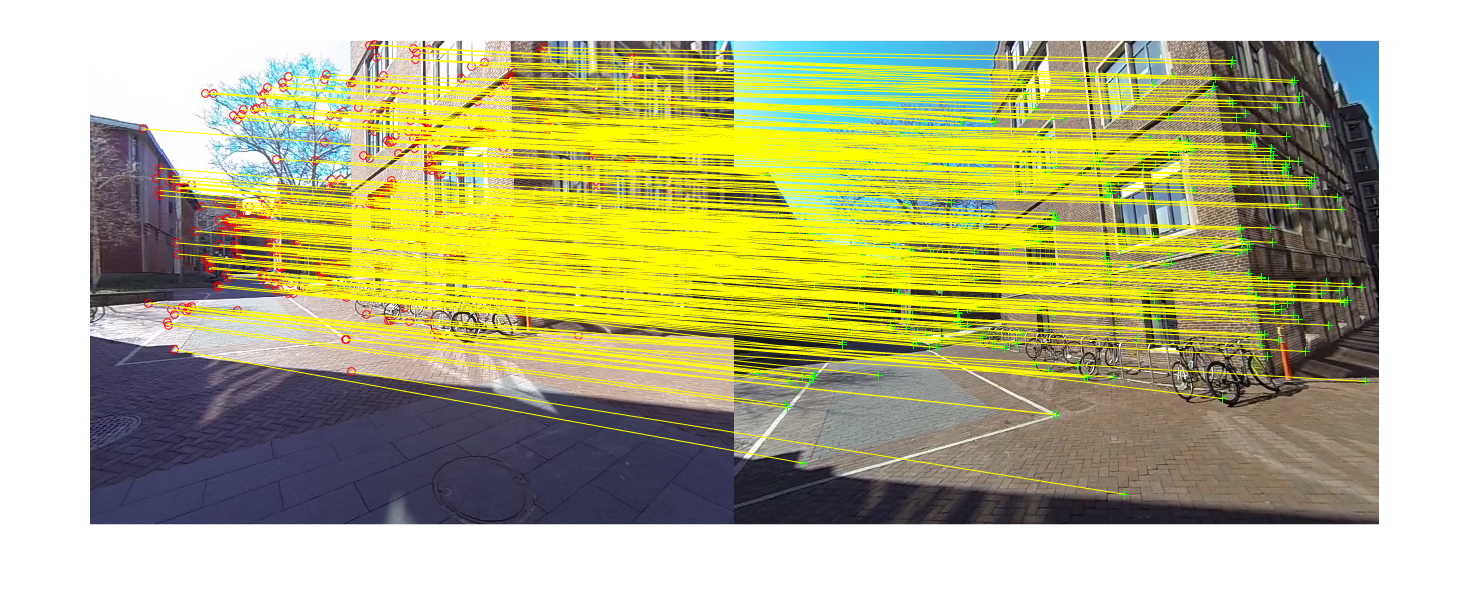
\includegraphics[width = \textwidth]{ransacmontage.png}
\caption{RANSAC matches shown across images 1 and 4}
\end{figure}


The Fundamental Matrix:

$$F = \begin{bmatrix}

   -0.0000   & 0.0000 &  -0.0089 \\
   -0.0000  &  0.0000   & 0.0032\\
    0.0131  & -0.0021  & -0.9999\\ \end{bmatrix}$$

Number of Inliers:\\
images 1 and 2. Percent inliers = 1.000000 \\
images 1 and 3. Percent inliers = 0.996711 \\
images 1 and 4. Percent inliers = 0.980851 \\
images 2 and 3. Percent inliers = 1.000000 \\
images 2 and 4. Percent inliers = 0.999068 \\
images 3 and 4. Percent inliers = 0.999564 \\
images 3 and 5. Percent inliers = 1.000000 \\
images 3 and 6. Percent inliers = 1.000000 \\
images 4 and 5. Percent inliers = 1.000000 \\
images 4 and 6. Percent inliers = 1.000000 \\
images 5 and 6. Percent inliers = 0.934351 \\


\section{Triangulation and Initial Camera Poses}
The Essential Matrix:
$$E = \begin{bmatrix}

   -0.0578  &  0.7054   & 0.0416\\
   -0.7503   & 0.0334  & -0.6579\\
    0.0019   & 0.7012 &   0.0938\\ \end{bmatrix} $$
\par
    
4 Possible Camera Poses:

$$C_1 = \begin{bmatrix}    
	-0.7052 \\
    0.0562\\
    0.7068\\
    \end{bmatrix}  $$
$$ R_1 = \begin{bmatrix}

   -0.0659  &  0.0533  & -0.9964\\
    0.0026  & -0.9986  & -0.0536\\
   -0.9978  & -0.0061  &  0.0657\\ \end{bmatrix} $$

$$C_2 = \begin{bmatrix}    
   -0.7052\\
    0.0562\\
    0.7068\\
    \end{bmatrix}  $$
$$ R_2 = \begin{bmatrix}

   -0.0659  &  0.0533  & -0.9964\\
    0.0026  & -0.9986  & -0.0536\\
   -0.9978  & -0.0061  &  0.0657\\ \end{bmatrix} $$
   
$$C_3 = \begin{bmatrix}    
    0.7052\\
   -0.0562\\
   -0.7068\\
    \end{bmatrix}  $$
$$ R_3 = \begin{bmatrix}

    0.9948    &0.0849  & -0.0559\\
   -0.0765   & 0.9876   & 0.1374\\
    0.0669   &-0.1324    &0.9889\\ \end{bmatrix} $$
    
$$C_4 = \begin{bmatrix}    
   -0.7052\\
    0.0562\\
    0.7068\\
    \end{bmatrix}  $$
$$ R_4 = \begin{bmatrix}

    0.9948   & 0.0849  & -0.0559\\
   -0.0765  &  0.9876   & 0.1374\\
    0.0669 &  -0.1324   & 0.9889\\ \end{bmatrix} $$
   
Camera Pose Configurations 3D Visual:

\begin{figure}[!h]
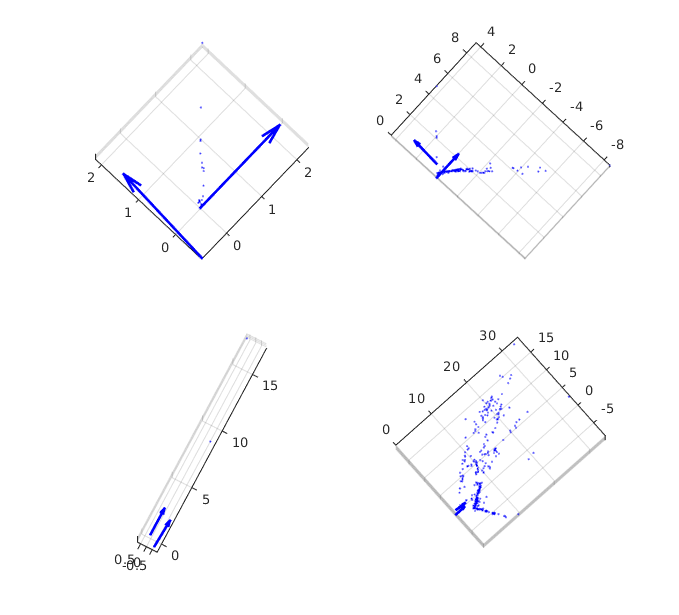
\includegraphics[width = \textwidth]{3dcamposes.png}
\centering
\caption{This visual shows the 4 camera poses with triangulated 3D points. Camera pose 4 was choosen.}
\end{figure}

\section{Nonlinear Triangulation}

Linear Triangulation compared to Nonlinear Triangulation:
\begin{figure}[!h]
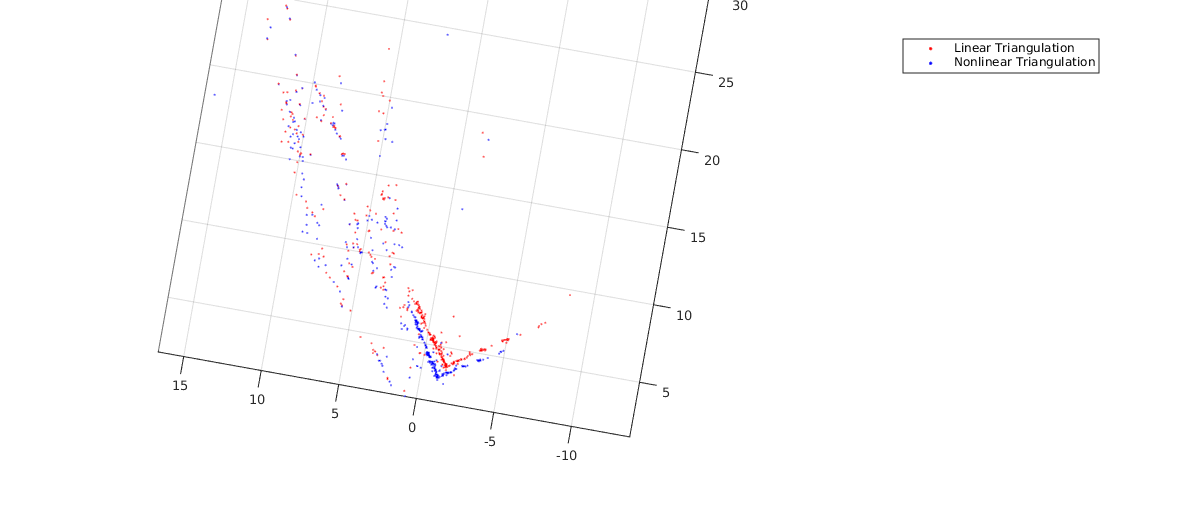
\includegraphics[width = \textwidth]{lvnl_top.png}
\centering
\caption{This visual shows non-linear and linear triangulation on the same plot. Top view.}
\end{figure}

Projections of Triangulations onto the Image:
\begin{figure}[!h]
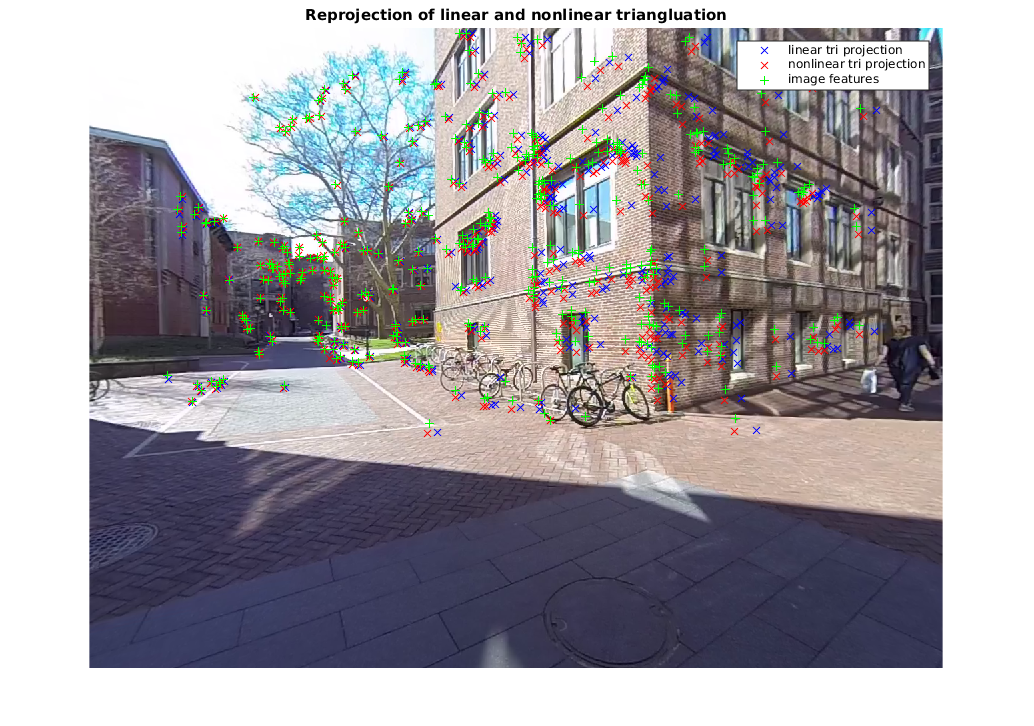
\includegraphics[width = \textwidth]{tri_proj_error.png}
\centering
\caption{This image shows the noticable difference between non-linear and linear triangualtion. It is more apparent in the right of the image.}
\end{figure}


\section{PnP RANSAC}
Camera Poses and Number of Inliers:
Camera 2:
$$C_2 = \begin{bmatrix}    
   -0.1561\\
   -0.0225\\
    0.2433\\
    \end{bmatrix}  $$
$$ R_2 = \begin{bmatrix}

	0.9740  &  0.0639  & -0.2173\\
   -0.0264  &  0.9849 &   0.1714\\
    0.2250  & -0.1612  &  0.9609\\ \end{bmatrix} $$
Kept 198 inliers of 198	Nonlinear PnP Points.
\\
Camera 3:
$$C_3 = \begin{bmatrix}    
   -0.4751\\
    0.0077\\
    0.4020\\
    \end{bmatrix}  $$
$$ R_3 = \begin{bmatrix}

    0.9986  &  0.0475 &  -0.0231\\
   -0.0431   & 0.9851 &   0.1664\\
    0.0306  & -0.1652 &   0.9858\\ \end{bmatrix} $$
Kept 661 inliers of 717	Nonlinear PnP Points.
\\
Camera 5:
$$C_5 = \begin{bmatrix}    
   -0.8299\\
    0.0783\\
    0.9752\\
    \end{bmatrix}  $$
$$ R_5 = \begin{bmatrix}

    0.9655  & -0.0208  & -0.2595\\
    0.0601  &  0.9877  &  0.1446\\
    0.2533  & -0.1552  &  0.9548\\ \end{bmatrix} $$
Kept 385 inliers of 421	Nonlinear PnP Points.\\
Camera 5:
$$C_5 = \begin{bmatrix}    
   -1.1776\\
    0.0628\\
    1.1814\\
    \end{bmatrix}  $$
$$ R_5 = \begin{bmatrix}

    0.9610  &  0.0534  & -0.2713\\
   -0.0066  &  0.9853  &  0.1706\\
    0.2764  & -0.1622  &  0.9473\\ \end{bmatrix} $$
Kept 478 inliers of 640	Nonlinear PnP Points.

Added Camera in 3D Reconstruction:
\begin{figure}[!h]
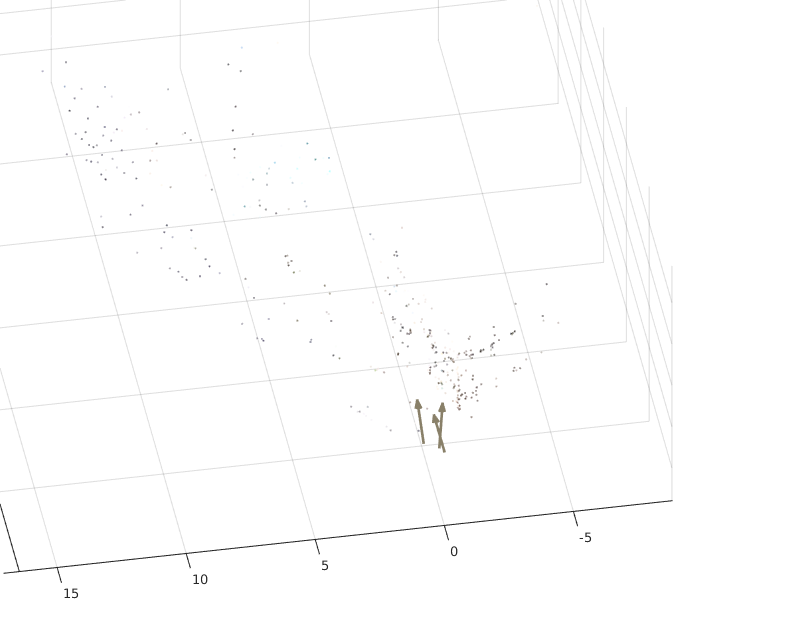
\includegraphics[width = \textwidth]{3dcampnp.png}
\centering
\caption{The cameras are shown as gray arrows. Notice they all point toward the structure starting to form.}
\end{figure}

\section{Nonlinear PNP}
2D Projection of 3D Points using Linear PNP and Nonlinear PNP Transforms:
\begin{figure}[!h]
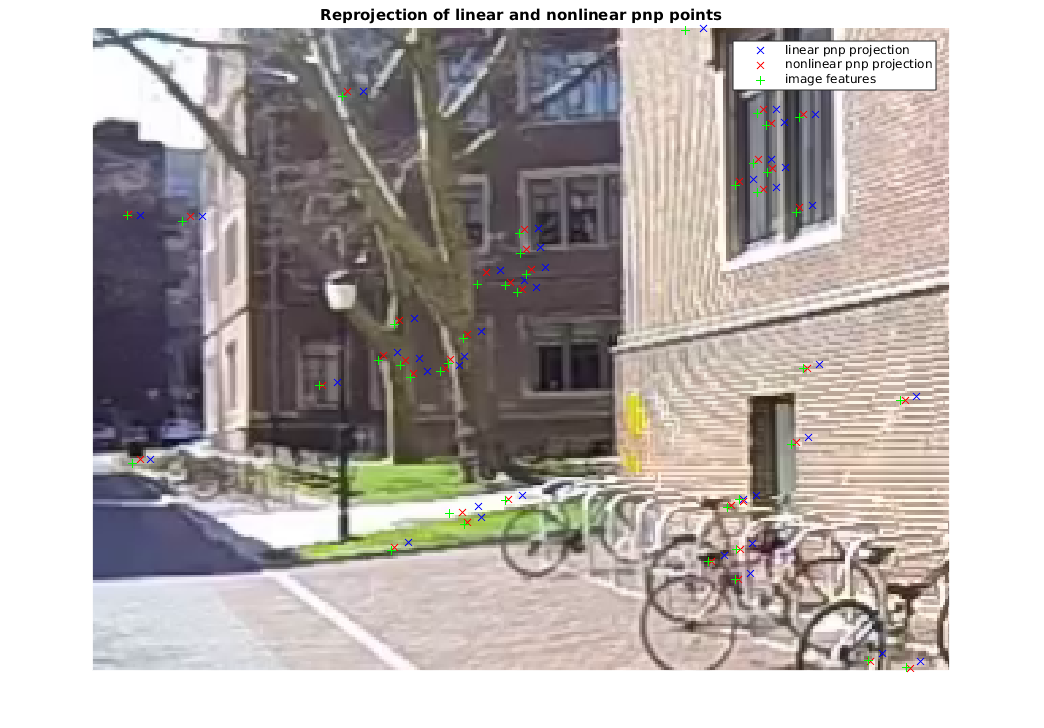
\includegraphics[width = \textwidth]{pnp_error_zoom.png}
\centering
\caption{This image is a zoomed in image to show to  projection errors. Notice the nonlinear PnP points are closer to to actual feature that the linear PnP points}
\end{figure}

\section{Bundle Adjustment}
The Final Bundle:
I was able to reconstruct all 6 cameras and 9971 points.
\begin{figure}[!h]
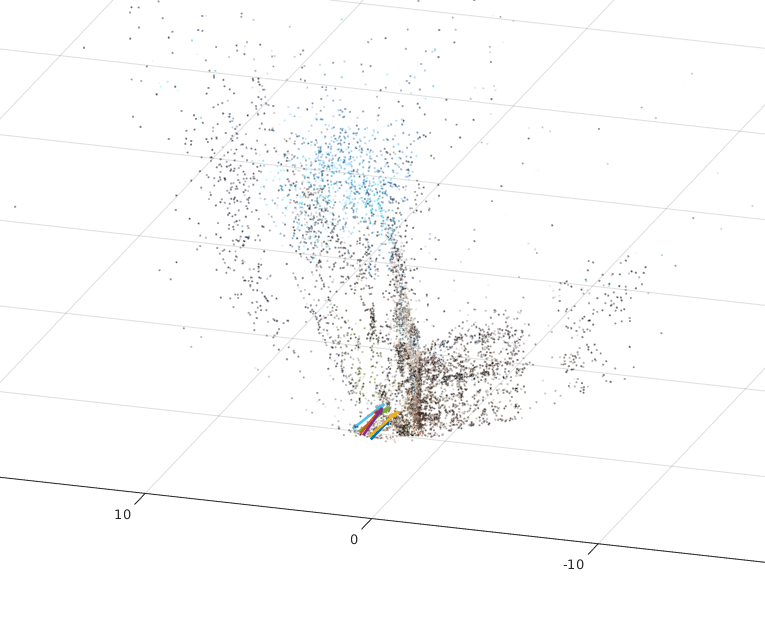
\includegraphics[width = \textwidth]{final_back.png}
\centering
\caption{This plot shows the final point cloud reconstruction with the colors mapped from the original images}
\end{figure}

\begin{figure}[!h]
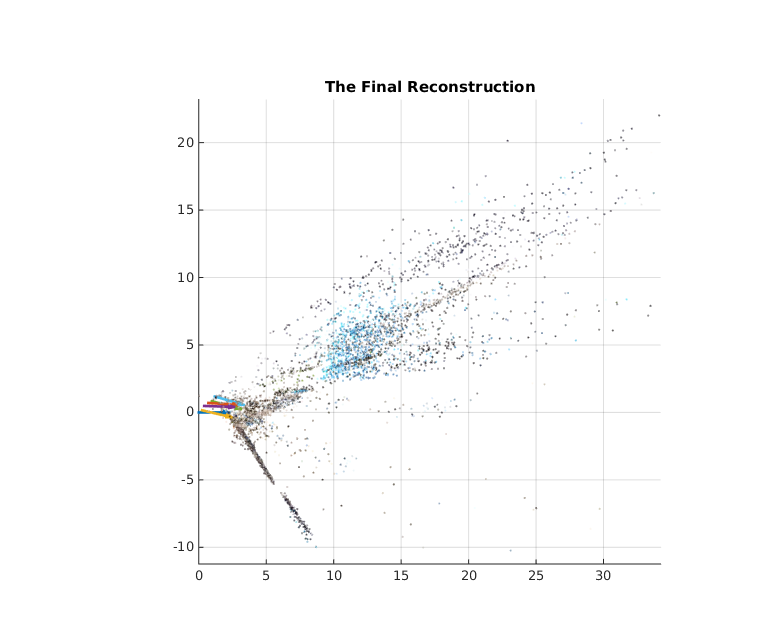
\includegraphics[width = \textwidth]{final_top.png}
\centering
\caption{This plot shows the final point cloud reconstruction with the colors mapped from the original images. top view.}
\end{figure}

2D Reprojections of 3D Points onto each Camera/Image:
\begin{figure}[!h]
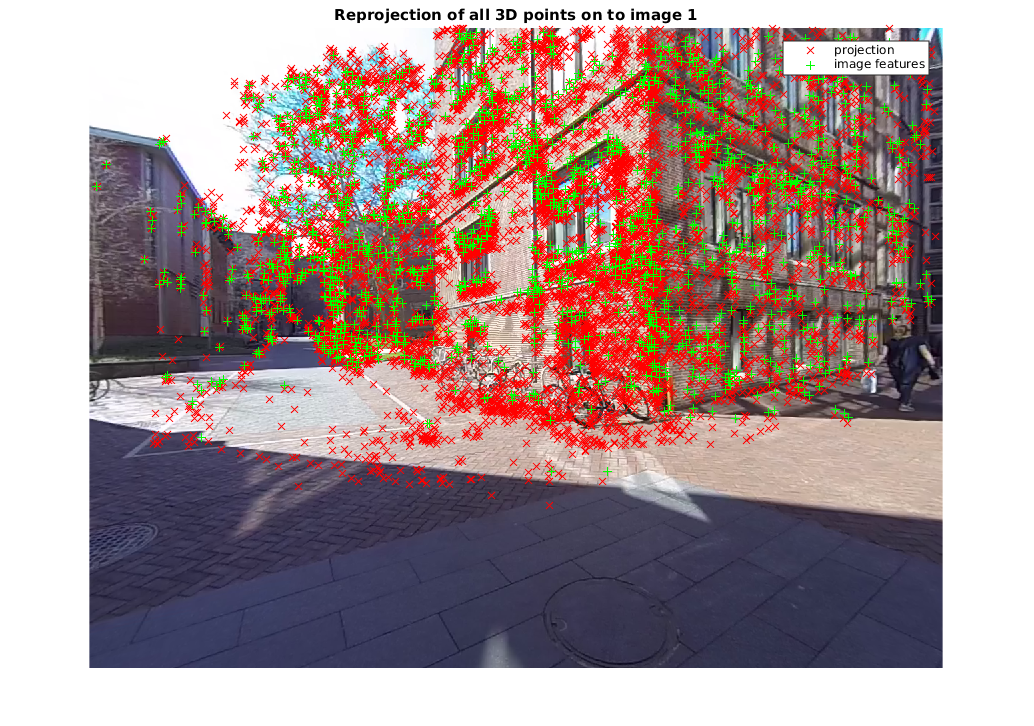
\includegraphics[width = \textwidth]{f1.png}
\centering
\caption{3D structure projection onto image 1}
\end{figure}
\begin{figure}[!h]
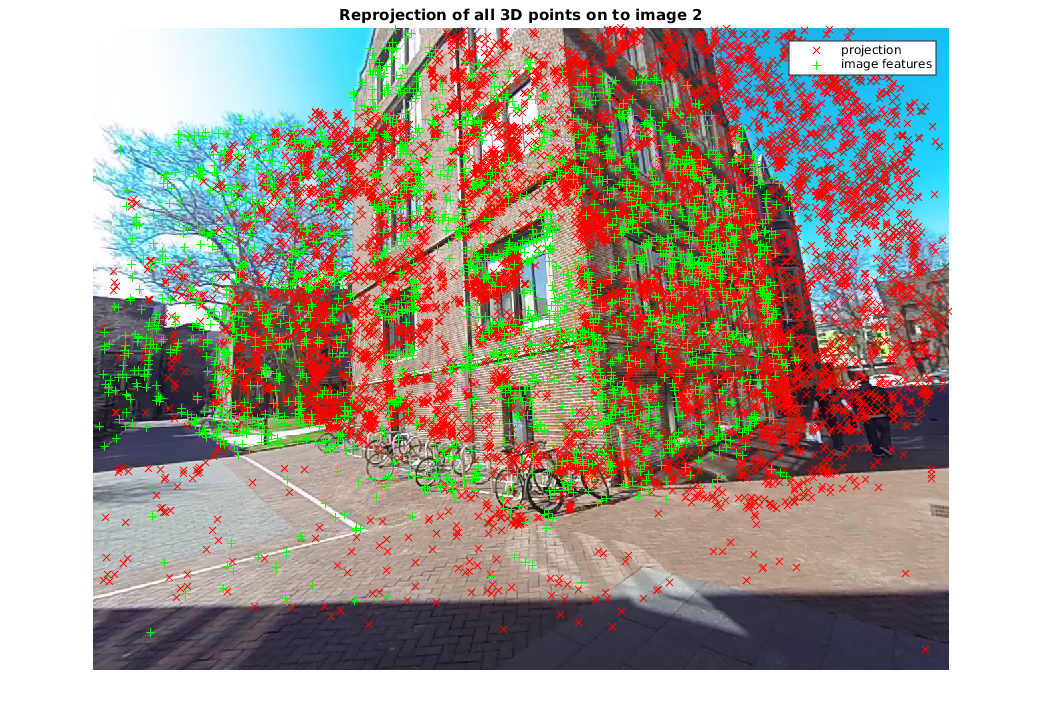
\includegraphics[width = \textwidth]{f2.png}
\centering
\caption{3D structure projection onto image 2}
\end{figure}
\begin{figure}[!h]
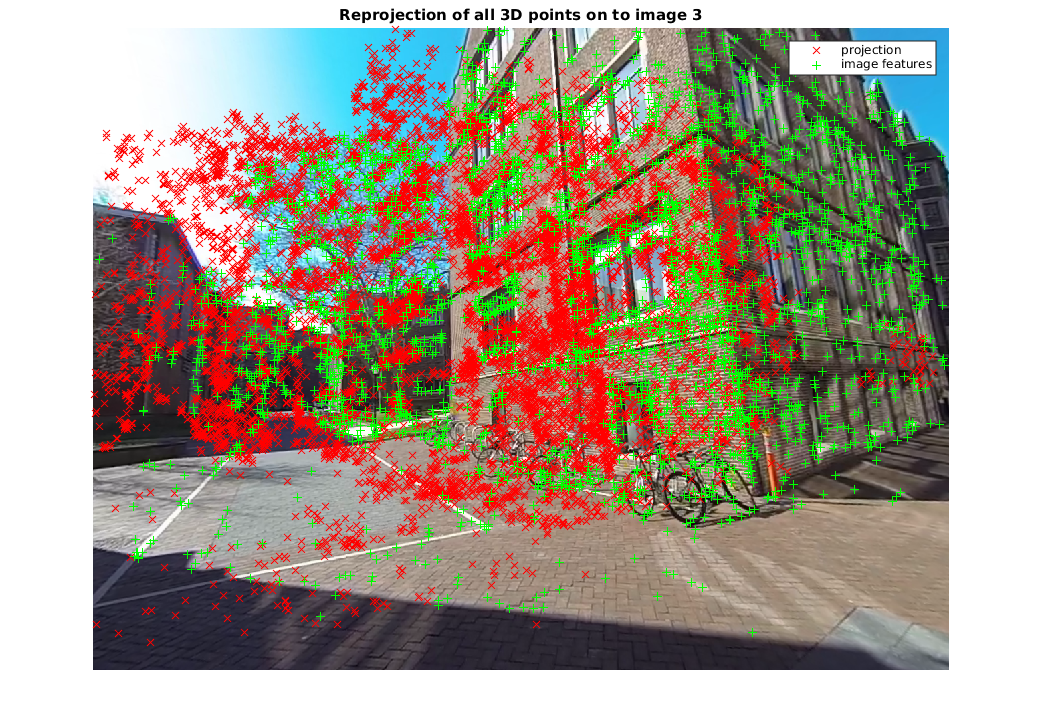
\includegraphics[width = \textwidth]{f3.png}
\centering
\caption{3D structure projection onto image 3}
\end{figure}
\begin{figure}[!h]
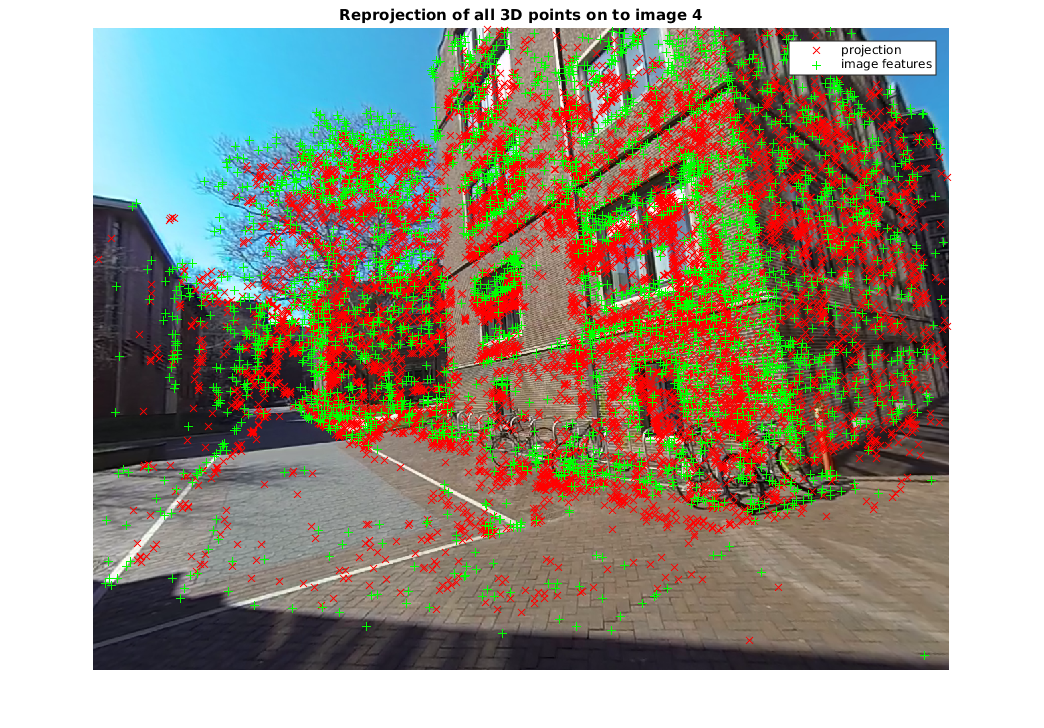
\includegraphics[width = \textwidth]{f4.png}
\centering
\caption{3D structure projection onto image 4}
\end{figure}
\begin{figure}[!h]
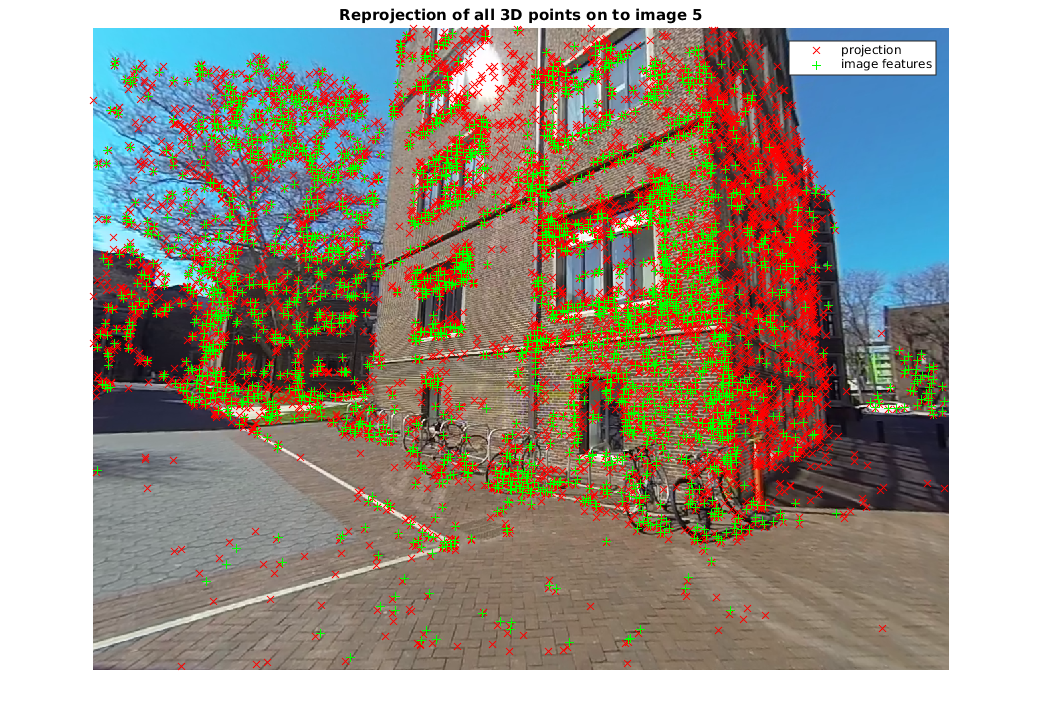
\includegraphics[width = \textwidth]{f5.png}
\centering
\caption{3D structure projection onto image 5}
\end{figure}
\begin{figure}[!h]
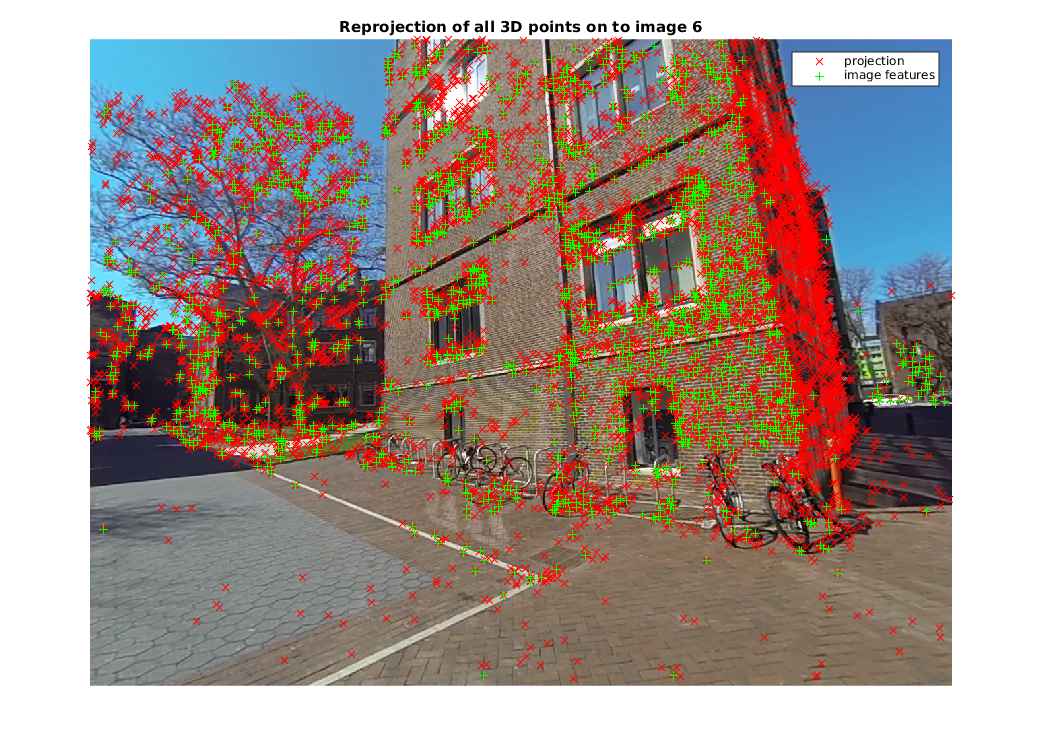
\includegraphics[width = \textwidth]{f6.png}
\centering
\caption{3D structure projection onto image 6}
\end{figure}

3D Point Cloud Colored by Camera:
\begin{figure}[!h]
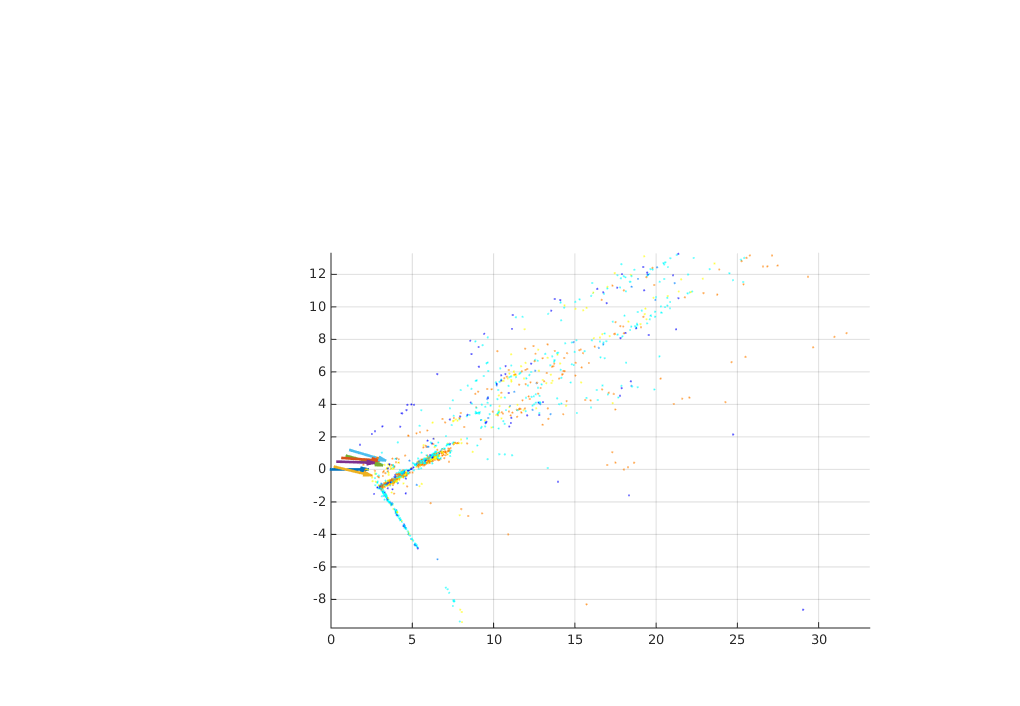
\includegraphics[width = \textwidth]{pointsbycam.png}
\centering
\caption{This plot shows which points were added by which camera. The point color matches the corresponding camera color.}
\end{figure}

\begin{figure}[!h]
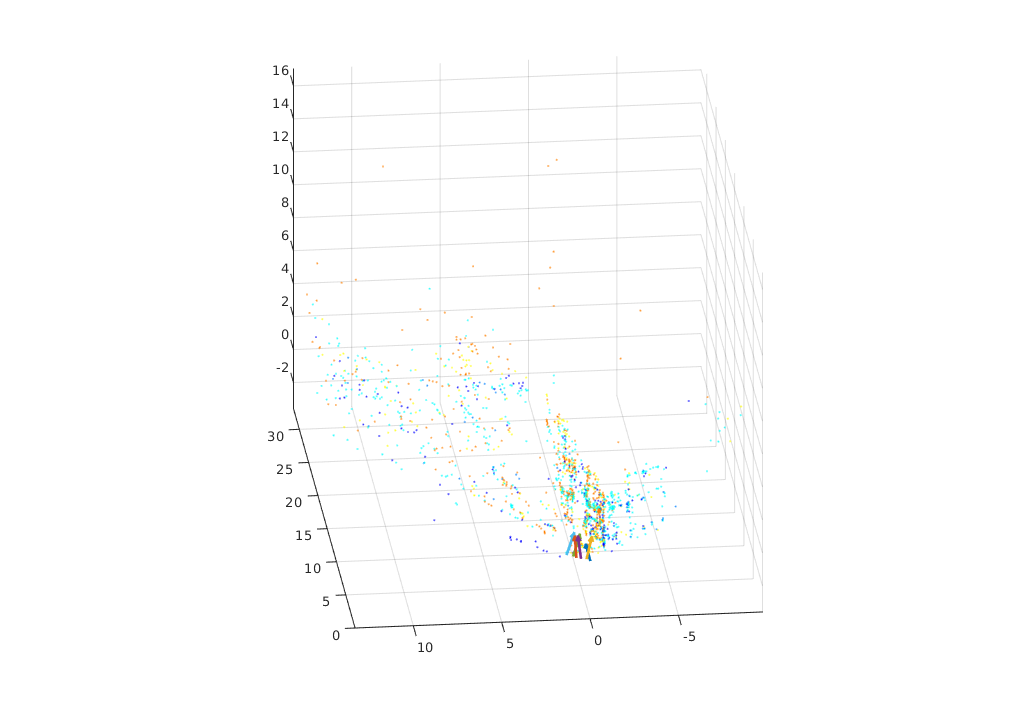
\includegraphics[width = \textwidth]{pointsbycam2.png}
\centering
\caption{This plot shows which points were added by which camera. The point color matches the corresponding camera color.}
\end{figure}




\end{document}